\let\negmedspace\undefined
\let\negthickspace\undefined
\documentclass[journal]{IEEEtran}
\usepackage[a5paper, margin=10mm, onecolumn]{geometry}
%\usepackage{lmodern} % Ensure lmodern is loaded for pdflatex
\usepackage{tfrupee} % Include tfrupee package

\setlength{\headheight}{1cm} % Set the height of the header box
\setlength{\headsep}{0mm}     % Set the distance between the header box and the top of the text

\usepackage{gvv-book}
\usepackage{gvv}
\usepackage{cite}
\usepackage{amsmath,amssymb,amsfonts,amsthm}
\usepackage{algorithmic}
\usepackage{graphicx}
\usepackage{textcomp}
\usepackage{xcolor}
\usepackage{txfonts}
\usepackage{listings}
\usepackage{enumitem}
\usepackage{mathtools}
\usepackage{gensymb}
\usepackage{comment}
\usepackage[breaklinks=true]{hyperref}
\usepackage{tkz-euclide} 
\usepackage{listings}
% \usepackage{gvv}                                        
\def\inputGnumericTable{} 
\usepackage[latin1]{inputenc}                                
\usepackage{color}                                            
\usepackage{array}                                            
\usepackage{longtable}                                       
\usepackage{calc}                                             
\usepackage{multirow}                                         
\usepackage{hhline}                                           
\usepackage{ifthen}                                           
\usepackage{lscape}

\begin{document}

\bibliographystyle{IEEEtran}
\vspace{3cm}

\title{1-1.10-24}
\author{EE24BTECH11006 - Arnav Mahishi}
% \maketitle
% \newpage
% \bigskip
{\let\newpage\relax\maketitle}

\renewcommand{\thefigure}{\theenumi}
\renewcommand{\thetable}{\theenumi}
\setlength{\intextsep}{10pt} % Space between text and floats


\numberwithin{equation}{enumi}
\numberwithin{figure}{enumi}
\renewcommand{\thetable}{\theenumi}
Question: Find the direction cosines of the unit vector perpendicular to the plane\\ $\overrightarrow{r}\cdot\brak{6\hat{i}-3\hat{j}-2\hat{k}}+1=0$\\
\begin{table}[h!]    
  \centering
  \begin{table}[H]
    \centering
    \begin{tabular}{|c|c|c|c|c|c|c|}
        \hline
        & \multicolumn{4}{c|}{\textbf{DESTINATIONS}} & \textbf{Supply} \\ \cline{2-5}
        \textbf{SOURCES} & P & Q & R & S & \\ \hline
        \textbf{1} & 13 & 8 & 12 & 9 & 20 \\ \hline
        \textbf{2} & 10 & 7 & 5 & 20 & 10 \\ \hline
        \textbf{3} & 3 & 19 & 5 & 12 & 50 \\ \hline
        \textbf{4} & 4 & 9 & 7 & 15 & 30 \\ \hline
        \textbf{5} & 14 & 0 & 1 & 7 & 40 \\ \hline
        \textbf{Demand} & 60 & 10 & 20 & 60 & \\ \hline
    \end{tabular}
\end{table} 

  \caption{Input Parameters}
\end{table}
\begin{align}
    \text{Soln: Comparing to form $\overrightarrow{r}\cdot\overrightarrow{n}=c$}\implies\overrightarrow{n}&=\myvec{6\\-3\\-2} \text{ and } c=-1\\
    \implies\abs{n}^2&=n^Tn=\myvec{6&-3&-2}\myvec{6\\-3\\-2}=49\\
    \implies\abs{n}&=7\\
    \implies\hat{n}&=\frac{\overrightarrow{n}}{\abs{\overrightarrow{n}}}=\frac{1}{7}\myvec{6\\-3\\-2}\\
    \therefore\text{DC's}&=\frac{6}{7},\frac{-3}{7},\frac{-2}{7}
\end{align}
\begin{figure}[h!]
   \centering
   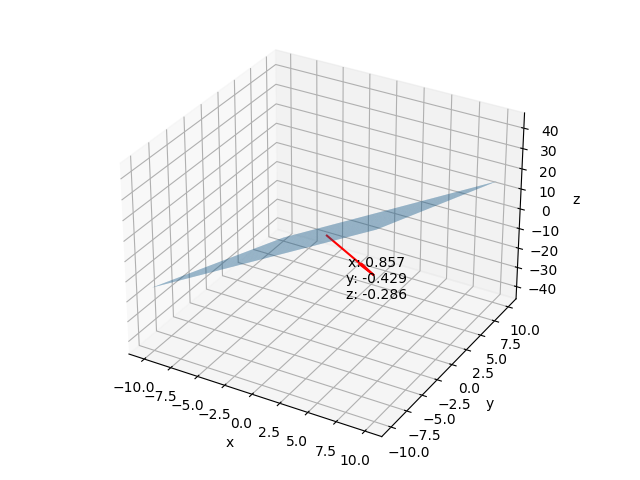
\includegraphics[width=0.7\linewidth]{figs/Figure_1.png}
   \caption{Plot of plane and normal vector}
   \label{stemplot}
\end{figure}
\end{document}
